
\documentclass{bredelebeamer}




%%%%%%%%%%%%%%%%%%%%%%%%%%%%%%%%%%%%%%%%%%%%%%%%



\title[Mini Project]{ XML INJECTION MUTATION FOR WEB SERVICES
	VULNERABILITY TESTING BASED ON SOAP
	MESSAGES}
% Titre du diaporama

%\subtitle{Vous pouvez ajouter un sous-titre}
% Sous-titre optionnel

\author{Bimal Varghese \\ %\inst{1}\\
		Simi Stephen  }%\inst{2}}
% La commande \inst{...} Permet d'afficher l' affiliation de l'intervenant.
% Si il y a plusieurs intervenants: Marcel Dupont\inst{1}, Roger Durand\inst{2}
% Il suffit alors d'ajouter un autre institut sur le modèle ci-dessous.

\institute[FISAT Mookkannoor]
{
%  \inst{1}%
  Federal Institute of Science and Technology \\
  Mookkannoor \\
  Angamaly
  }


\date{18 May 2015}
% Optionnel. La date, généralement celle du jour de la conférence

%\subject{Sujet de votre diaporama}
% C'est utilisé dans les métadonnes du PDF



%\logo{
%
\includegraphics[scale=0.15]{images/logo.png}
%}



%%%%%%%%%%%%%%%%%%%%%%%%%%%%%%%%%%%%%%%%%%%%%%%%%%%%%%%%%%%%%%%%%%%%%
\begin{document}

\begin{frame}
  \titlepage
\end{frame}





\begin{frame}{Outline}
  \tableofcontents
  % possibilité d'ajouter l'option [pausesections]
\end{frame}




\section{INTRODUCTION}

\begin{frame}
	\centering{ \huge \textbf{INTRODUCTION}}
\end{frame}

\subsection{Web Service}
\begin{frame}{Web Service}
	\large
	 \begin{itemize}
	 	\item Common way of implementing SOA.
	 	\newline
	 	
	 	\item Widely used in the Internet. 
	 	\newline
	 	\item Good Encapsulation and Strong Integration capabilities making it more useful.
	 	\newline
	 	\item Architecture of Web Service may cause security vulnerabilities.
	 	\newline
	 	\begin{itemize}
	 		\large
	 		\item Quality and Reliability of Web Service must be heavily tested.
	 	\end{itemize}
	  	
	 \end{itemize}
\end{frame}

\subsection{Vulnerability Testing of Web Service}
\begin{frame}{Vulnerability Testing of Web Service}
	\large
	\begin{itemize}
		\item Components in WS.
		\newline
		\begin{itemize}
			\large
			\item WSDL.
			\item SOAP.
			\item XML.
			\item UDDI.
			\newline
			\pause
		\end{itemize}
	
		\item Vulnerability refers to flaws in the service that threaten the security of
		the Application/computer system.
		\newline
		\item Traditional Software testing methods may not work with Webs Services. 
		\begin{itemize}
			\large
			\item Heterogeneous nature. 
			\item Lack of User Interface (UI).
		\end{itemize}
	\end{itemize}
\end{frame}
\begin{frame}{Difficulties in Testing Web Service}
	\large
	

	\begin{block}{Factors that contributing to
			the difficulty of Web Service Testing}
	\begin{enumerate}
		\large
		\item Different development and application environments.
		\newline
		\item The characteristics of Web service distribution, discovery, and dynamic bindings.
		\newline
		\item The need for a service interface for Web service design and implementation when
		applying automatic testing methods and techniques
	\end{enumerate}
	\end{block}
\end{frame}


\begin{frame}
	\begin{block}{Shortcommings in Web Service Testing}
	\begin{itemize}
		\large
		\item The need
		for significant human intervention in the process.
		\newline
		\item Simple performance
		and access testing have been performed.
		\newline
		\item Extensible Markup Language (XML)
		in web service considered only for data transmission and not of data storage 
	\end{itemize}
	\end{block}
\end{frame}

\section{LITERATURE SURVEY}
\begin{frame}
	
  \centering{\huge \textbf{Literature Survey}}
	
\end{frame}


\begin{frame}{[1] Automated Robustness Testing of Web Service}
	Presents a framework for automatically generating and
	execution of web service.
	
	\begin{block}{Method}
		\begin{enumerate}
			\large
			\item Code Generator
			
			\begin{enumerate}
				\large
				\item Generate necessary code to implement a service consumer
				\newline
			\end{enumerate}
			
			\item Test Generation
			
			\begin{enumerate}
				\large
				\item Generated test class is supplied to a test generation tool such as JCrasher inorder to generate JUnit test.
				\newline
			\end{enumerate}		
			
			\item Test Execution
			
			\begin{itemize}
				\large
				\item Invoke test case and call web service.
				Collect response from web service.
				\newline
			\end{itemize}
			
		\end{enumerate}
	\end{block}
	
\end{frame}


%\begin{frame}{[2] Extending WSDL to Facilitate Web Services Testing}
%
%	
%%	\begin{block}{Method}
%		\begin{itemize}
%			\large
%			\item Object Oriented Framework for testing.\newline
%			\item To perform black-box testing and regression testing, some additional information regarding the web service is required which include.
%			
%			\begin{enumerate}
%				\large
%				\item Input-output Dependency : by introducing complex type in WSDL schema, WSIOPairType 
%				\newline
%				\item Invocation Sequences : to trace and state the
%				calling relationship of web services,  MtSS (Method Sequence 
%				Specification) was utilized.
%				\newline
%				\item Hierarchical Functional Description :  to 
%				incorporate functional descriptions into WSD, two sub-elements WSFParents and WSFChild are added.
%				\newline
%				\item Concurrent Sequence Specifications : to capture calling sequences in Object Oriented 
%				frameworks.
%				\newline
%			\end{enumerate}
%			
%			
%			
%		\end{itemize}
%%	\end{block}
%	
%\end{frame}


\begin{frame}{[2] Exploring Perturbation Based Testing for Web
		Service}
	\begin{itemize}
		\large
		\item Extended approach based on XML message perturbation
		\newline
		\item Utilized SOAP Perturbation operators and a Web service Testing
		tool ( SMAT-WS )
		\newline
		\begin{block}{SOAP Perturbation Operator}
			SOAP perturbation primitive operators include.
			\begin{enumerate}
				\large
				\item  \textit{Null (n)}
				\item \textit{Incomplete (n)}
				\item \textit{Inversion (n)}
				\item \textit{ValueInversion (n)}
				\item \textit{Mod\_Len (n)}
				\item \textit{Space (n)}
				
			\end{enumerate}   
		\end{block}
	\end{itemize}
\end{frame}

\begin{frame}{[3] Efficient Web Services Message Exchange by SOAP Bundling Framework}
	\begin{block}{}
		\large
		\begin{itemize}
			\item A SOAP message bundling framework is Proposed.
			\newline
			\item Framework enables bundling of multiple messages into one message.
			\newline
			\item Application developers do not have to consider the service granularity for performance reasons.
			\newline
		\end{itemize}
	\end{block}
\end{frame}

\begin{frame}{[4] Generating Test Cases for Web Services Using Data Perturbation}
	\begin{itemize}
		\large
		\item Existing XML messages are modified based on rules defined on the message grammars, and then used as tests.
		\newline
		\item Data perturbation uses 2 methods to test Web services:\\
%		\newline
		 \textbf{Data value perturbation}:\\ modifies values according to the data type.
		 \newline
		 \textbf{Interaction perturbation}:.\\classifies the communication messages into two categories: RPC communication and data communication
		
	\end{itemize}
\end{frame}

\begin{frame}{[5] Adaptive Random Testing: the ART of Test Case Diversity}
	
	
	\begin{block}{Base Idea}
		
		\begin{itemize}
			\LARGE
			\item Many program faults result in failures at contiguous areas of the input domain - failure patterns.\newline
			\item For detecting failure patterns, ART systematically filters randomly generated candidates.
		\end{itemize}
	\end{block}
\end{frame}


\begin{frame}{Contd\dots}
	\begin{block}{Adaptive Random Testing}
		\textbf{Principle}
		\begin{itemize}
			\large
			\item Given a set of previously executed test cases
			that have not revealed any failures, new test cases
			located away from these old ones are more likely to
			reveal failures.
		\end{itemize}
		\textbf{Types of ART methods}
		\begin{itemize}
			\large
			\item Fixed Size Candidate Set ART (FSCS-ART):\\
			Candidate with largest distance from current Test case is considered next.
			\item Restricted Random Testing (RRT):\\
			Create Exclusion zone for current test case.\\
			Take random selection if it lie outside the zone.
		\end{itemize}
		
	\end{block}
\end{frame}
%\begin{frame}{Contd\dots}
%	\begin{block}{Identifying Failure Pattern using ART}
%		\begin{enumerate}
%			\large
%			\item Take samples from the set of all possible inputs to the software under test.\newline
%			\item Execute samples one by one, and determine whether the outputs from each sample match the software specification.\newline
%			\item If not, a software failure is revealed and existence of fault is detected.\newline
%			\item Select test data so as to maximize the number of distinct faults detected.
%		\end{enumerate}
%	\end{block}
%\end{frame}

\begin{frame}{[6] Testing Web Services by XML Perturbation}
	\begin{itemize}
		\large
		\item Web services uses XML to describe and transmit data.
		\newline
		\item XML schema is utilized to generate data formats and test cases.\newline
		\item Some applications and web services do not validate XML messages against an XML schema, and sometimes no schema exists.
		
	\end{itemize}
	
\end{frame}

\begin{frame}{Contd\dots}
	\begin{block}{XML Data Model}
		\begin{itemize}
			\large
			\item An XML schema can be modeled as a tree.
			\newline
			
			
			XML tree T = (N, D, X, E, $n_r$ ), where:\\
			\begin{itemize}
				\large
				\item N is a finite set of elements and attribute nodes.
				\item D is a finite set of built-in and derived data types.
				\item X is a finite set of constraints (integrity and representation).
				\item E is a finite set of edges.
				
				\item   $n_r$ is the root node.
			\end{itemize}
			
		\end{itemize}
	\end{block}
\end{frame}
\begin{frame}{[7] Combinatorial Mutation Approach to Web Service Vulnerability Testing }
	\large
	Combinatorial mutation
	testing focuses on using combinations of at least two faulty
	input data parameter to find faults within the software.\newline
	\begin{itemize}
		\large
		\item A set of operators that can be combined are presented
		\item SOAP message is obtained by parsing the WSDL file, and data perturbation techniques are adopted to generate simple initial test data.
		\item A combinatorial testing method is developed.
	\end{itemize}
	
\end{frame}
\begin{frame}{Contd\dots}
	
	
	\begin{block}{Mutation Operator Design}
		\large
		Two perturbation policies which directly act on the SOAP message are used\newline
		\begin{itemize}
			\large
			\item Data Value perturbation :\\
			modifies
			values in SOAP messages according to their data types\newline
			\item Interaction perturbation :\\
			consider the data values and data relationships
		\end{itemize}
	\end{block}
\end{frame}

\begin{frame}{[8] Worst-Input Mutation Approach to Web Services Vulnerability Testing Based on SOAP Messages}
	\large
	Proposed Worst Input Mutation approach based on SOAP message mutation.
	\begin{block}{Method}
		\begin{itemize}
			\large
			\item Worst Input Mutation:\\
			Utilizing characteristics of SOAP message.
			\item Automatic Test Case Generation:\\
			Test Case Generation based on Farthest Neighbor (TCFN) algorithm
			\item A prototype Web Service Vulnerability Testing Tool is implemented
		\end{itemize}
	\end{block}
\end{frame}


\subsection{METHODS COMPARISON}
\begin{table}[H]
	\small
	\caption{Comparison of various Testing Approaches}
	\begin{tabular} {|m{.40cm}|m{3cm} | m{3.2cm} | m{3.0cm}|} %{|c|c|c|c|}
		\hline \textbf{Sl.No} & \textbf{Paper} & \textbf{Approach} & \textbf{Technology}  \\ 
		\hline 1 & Automated Robustness Testing of Web Service & Automatic code generator and testing framework & Existing java Technology \\
%		\hline 2 & Extending WSDL to Facilitate Web Services
%		Testing  &  XML-based object-oriented testing framework & OWL-S (Web ontology language for Web services)  \\ 
		\hline 2 & Exploring Perturbation Based Testing for Web
		Service & XML message perturbation & SOAP Perturbation operators   \\ 
		\hline 3 & Efficient Web Services Message Exchange
		by SOAP Bundling Framework & Multiple message bundling  & SOAP message bundling framework  \\ 
		\hline 4 & Generating Test Cases for Web Services Using Data Perturbation & Data perturbation & RPC and Data communication \\ 
		\hline 5 & Adaptive Random Testing: the ART of Test
		Case Diversity &  Fixed Size Candidate Set ART (FSCS-ART) 
		
		Restricted Random Testing (RRT) & Random candidate generation  \\ 
		\hline 6 & Testing Web Services by XML Perturbation & XML schema perturbation  & XML Tree Data Model  \\ 
		\hline 7 & Combinatorial Mutation Approach to Web
		Service Vulnerability Testing & Combinations of at
		least two faulty input data parameter to find faults  & SOAP message mutation  \\ 
		\hline 8 & Worst-Input Mutation Approach to Web Services Vulnerability Testing Based on SOAP Messages & Farthest Neighbor Approach & SOAP message mutation \\
		\hline 
	\end{tabular} 
\end{table}
\framebreak
\section{METHODOLOGY}
\begin{frame}
	
	\centering{\LARGE \textbf{METHODOLOGY}}
	
\end{frame}


\begin{frame}{Current Scenario}
	\begin{itemize}
		\large
		\item Test case generation :- An effective way of testing the credibility of Softwares.
		\newline
		\item Web Service components depend mainly on XML.
		\newline
		\item Both WSDL \& SOAP component of Web service depend on XML.  
		\newline
		\item Efficient Test cases for Web Service depends on XML.
		\newline
		\item Efficient mutation of XML will be an effective Test case.  
		\newline
	\end{itemize}
\end{frame}

\subsection{SOAP message muatation}
\begin{frame}{SOAP message muatation}
	\begin{itemize}
		\large
		\item Existing SOAP message mutation drawbacks are.
		\newline
		\begin{itemize}
			\large
			\item Redundancy of data in the SOAP message.
			\newline
			\item Low efficiency of the mutation operators.
			\newline
			\item  One mutant injected
			at one time
			\newline
		\end{itemize} 
	\end{itemize}
\end{frame}

\subsection{Mutation Operators}
\begin{frame}{Mutation Operators}
	\begin{itemize}
		\large
		\item Based on SOAP messages.
		\newline
		\item XML model for SOAP message can be considered as an Extended Regular Tree Grammar. 
		\newline
		\item eRTG (extended RTG) contains 6 tuples  $ < E; N; DT; P; A; n_{s} >  $
		\begin{itemize}
			\large
			\item E is a finite set of elements;
			\item N is a finite set of non-terminals
			\item DT is a finite set of data types {int, string, bool, numerical, char, object}
			\item P is a finite set of production rules
			\item $ n_{s} $ is the starting non-terminal
			\item A is a 2-tuple $ < n; type > $  n - number of parameters and ``type” - parameter type.
		\end{itemize}
%		\newline
	\end{itemize}
\end{frame}

\begin{frame}{Cont \dots}
	\large
	Given a set of all element instances N
	\newline
	\begin{itemize}
		\large
		\item Mutation operator r = $ f(n_{1}, n_{2}, ...n_{i}) $.
		\newline
		\begin{itemize}
			\large
			\item f - a function.
			\newline
			\item $ (n_{1}, n_{2}, ...n_{i}) \epsilon N  $ for i $ \geq $ 1 with arbitrary data type. 
			\newline
			\item r outputs mutated  $ (n_{1}, n_{2}, ...n_{i})$ with the same data type as the input  $ (n_{1}, n_{2}, ...n_{i})$
			\newline
		\end{itemize}
	\end{itemize}
\end{frame}


\begin{frame}
	\large 
	\begin{block}{
			Security rule for testing the vulnerability of Web services.}
%	\newline
	\begin{itemize}
		\large
		\item  VWS = $ G(r) $, where r=$ f(n_{1}, n_{2}, ..., n_{i}) $ is the mutation operator for the tested Web service
		\newline
		 \item G(r) the vulnerability that is triggered by r
		 \newline 
		 \item  $ n_{i} \epsilon N $ the Web service input parameters.
	\end{itemize}
	\end{block}
	\begin{figure}
\centering
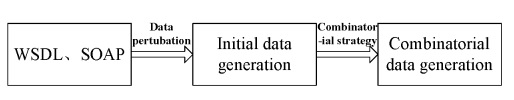
\includegraphics[width=0.5\linewidth]{images/WS/Fig1}
\caption{Steps to generate combinatorial data to Web service vulnerability testing}
\label{fig:Fig1}
\end{figure}
	
\end{frame}


\subsection{Worload Generation}
\begin{frame}{Workload Generation}
	\begin{itemize}
		\large
		\item Specific
		workload for each service need to be generated.
		\newline
		\item Workload is generated based on the following steps:
		\newline
		
			\begin{enumerate}
				\large
				\item Generate test values for each input parameter
				\newline
				\item Generate test calls for each operations
				\newline
				\item Execute call for each operation
			\end{enumerate}
		
	\end{itemize}
\end{frame}

\subsection{Attackload Generation}
\begin{frame}{Attackload Generation}
	
	\begin{itemize}
		\large
		\item Based on number and type of SOAP message parameters, input domain is partitioned.
		\newline
		\item Corresponding test case is then selected. 
		\newline
	\end{itemize}
	\begin{figure}
\centering
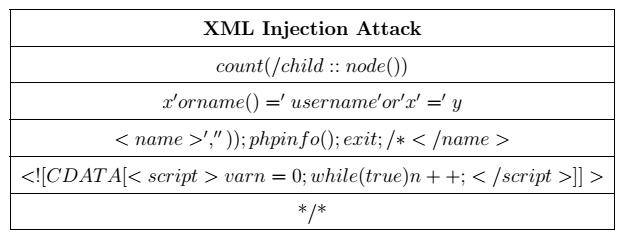
\includegraphics[width=0.7\linewidth]{images/WS/AttackLoad}
\caption{Examples of XML Injection Attack Loads}
\label{fig:AttackLoad}
\end{figure}
\end{frame}

%\subsection{Combinatorial Testing Strategy}
%\begin{frame}{Combinatorial Testing Strategy}
%	\begin{itemize}
%		\large
%		\item Step 1:Analyze and identify Web service methods and   associated methods with it.
%		\newline
%		\item Step 2: Invoke different sets of mutation operators according to the type of parameters.
%		\newline
%		\begin{itemize}
%			\item  Parameter set PS is formed,
%			denoted by PS= $ \{ p_{1}, p_{2}, ...p_{i}, q_{1}, q_{2}, ..., q_{j} \} $. 
%			\newline
%		\end{itemize}
%		
%	\end{itemize}
%\end{frame}

\begin{frame}
	\large
	Specific Combinatorial Methods are
	\newline
	\begin{itemize}
		\large
		\item \textit{Data Value Perturbation:} intended
		to check the integrity of data validity of the system.
		\newline
		\begin{itemize}		
		\item The combinatorial test
		data are generated by calling minimum K factors (K=2) of PS
		\newline
		\end{itemize}
		
		\item \textit{Interaction Perturbation :}  To check the integrity of the various interaction mechanism such as data retrieval and communications between the system.\newline
		\begin{itemize}		
		\item Based on the faults generally occurring among the parameters of the adjacent locality principle, $ k=\lceil(i+j)/2 \rceil $
		\end{itemize}
	\end{itemize}
\end{frame}

\section{EXPERIMENTAL RESULTS}
\begin{frame}
	\centering{ \huge \textbf{EXPERIMENTAL RESULTS}}
\end{frame}

\begin{frame}{Experimental implementation}
	Web service vulnerability testing system (WSVTS) is implemented in C\# 
	\begin{figure}
\centering
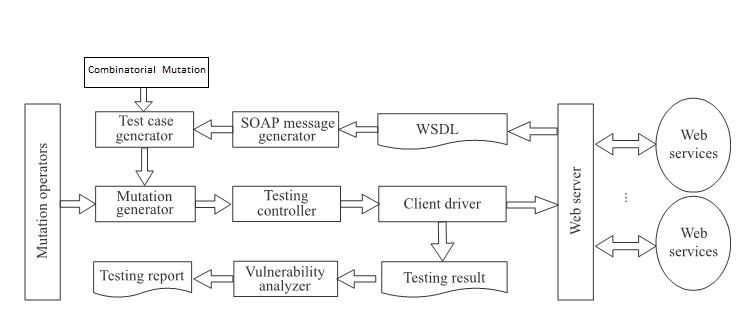
\includegraphics[width=0.9\linewidth]{images/WS/Fig3}
\caption{The WSVTS framework.}
\label{fig:Fig3}
\end{figure}

\end{frame}

\begin{frame}
	Four main function modules
	\newline
	\begin{enumerate}
		\large
		\item SOAP message generator
		\newline
		\item SOAP message mutation generator
		\newline
		\item Test case generator
		\newline
		\item Vulnerability analyzer
		\newline
	\end{enumerate}
\end{frame}


\begin{frame}
	
	\begin{figure}
\centering
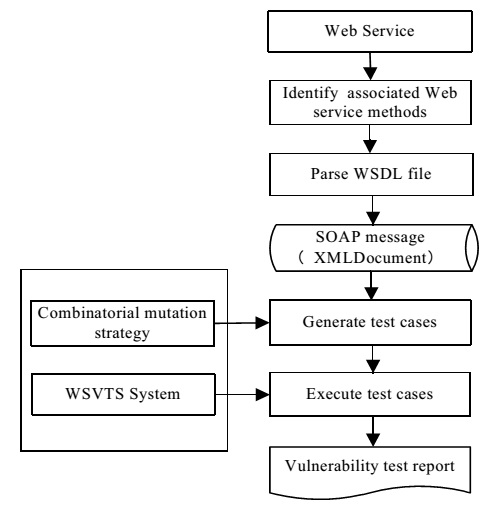
\includegraphics[width=0.5\linewidth]{images/WS/Fig4}
\caption{Flow chart of the Web Service vulnerability testing system}
\label{fig:Fig4}
\end{figure}

	
\end{frame}

\begin{frame}
	
	\begin{figure}
\centering
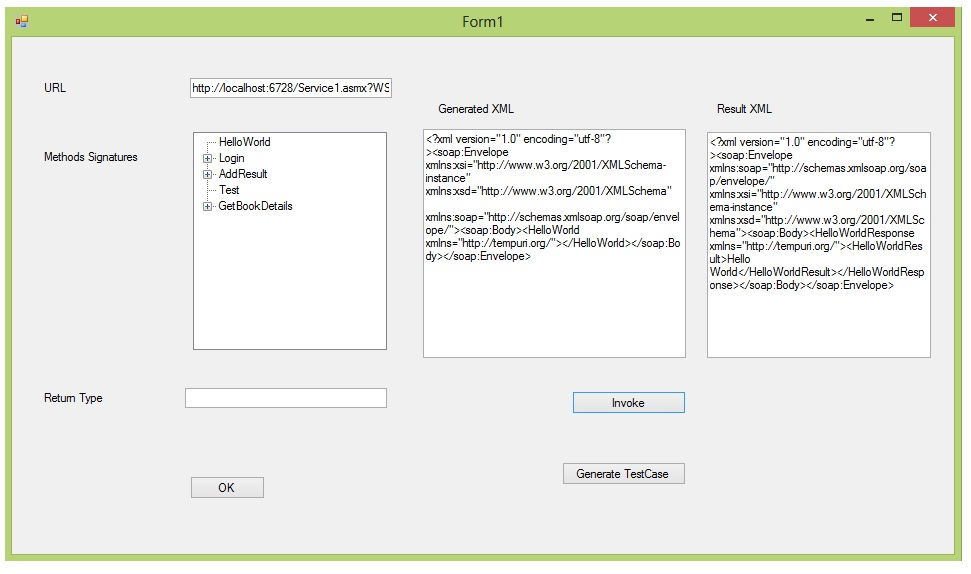
\includegraphics[width=0.7\linewidth]{images/WS/Fig7}
\caption{Simple Test case using WSVTS}
\label{fig:Fig7}
\end{figure}

	
\end{frame}

\begin{frame}
\begin{figure}
\centering
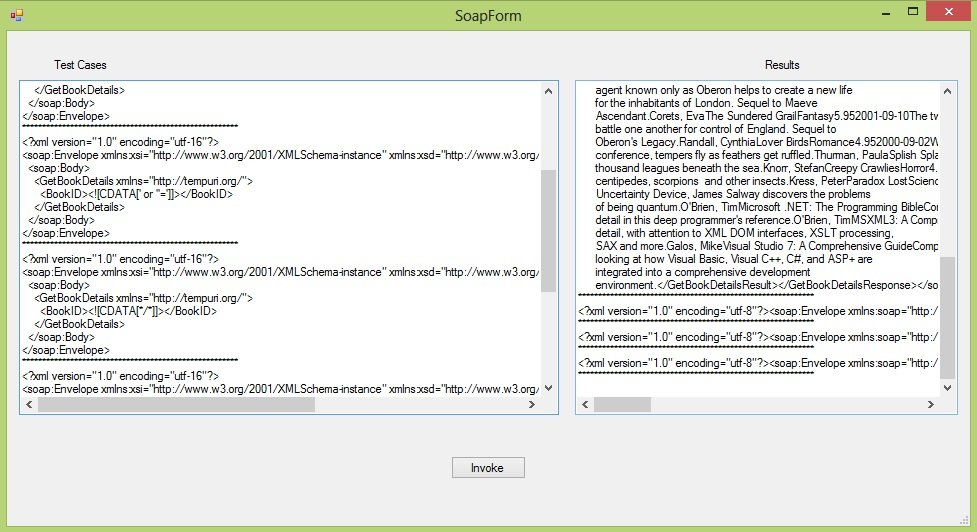
\includegraphics[width=0.7\linewidth]{images/WS/Fig8}
\caption{Combinatorial Test cases for XML injection 1}
\label{fig:Fig8}
\end{figure}

\end{frame}

\begin{frame}
\begin{figure}
\centering
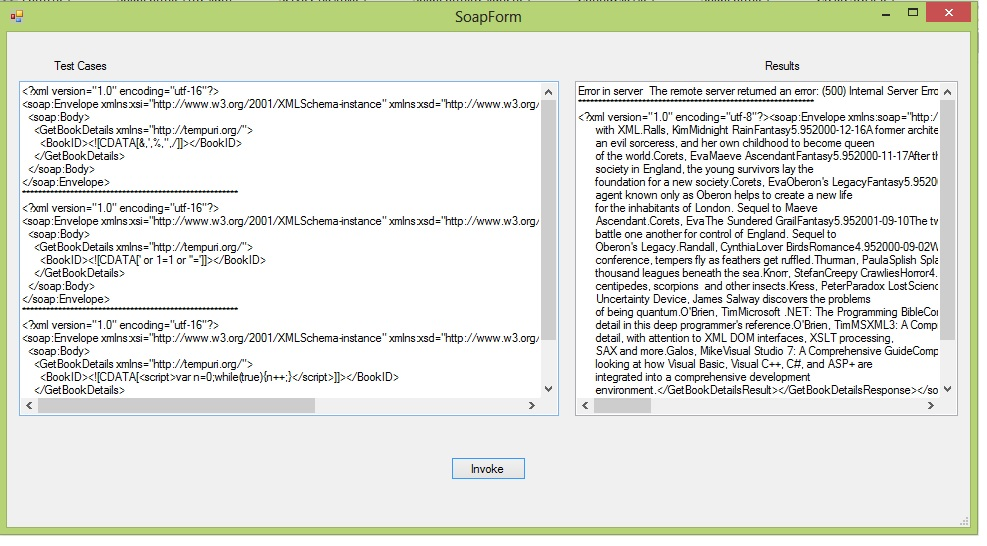
\includegraphics[width=0.7\linewidth]{images/WS/Mut1}
\caption{Combinatorial Test cases for XML injection 2}
\label{fig:Mut1}
\end{figure}

\end{frame}

\begin{frame}{Comparison with other system}

\begin{figure}
\centering
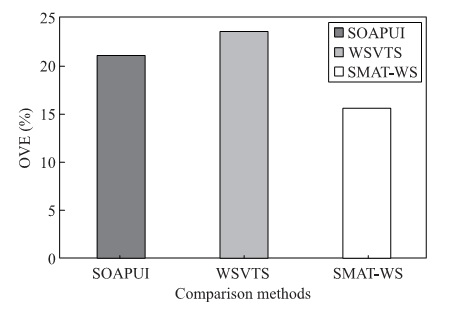
\includegraphics[width=0.7\linewidth]{images/WS/Fig11}
\caption{Comparison of the overall efficiency of SOAPUI, WSVTS, SMAT-WS.}
\label{fig:Fig11}
\end{figure}

\end{frame}

\section{CONCLUSION}
\begin{frame}
	\centering{ \huge \textbf{CONCLUSION}}
\end{frame}


\begin{frame}
	\begin{itemize}
		\large
		\item Due to specific nature of Web services, traditional software testing techniques cannot be completely adopted
		to test Web services.
		\newline
		\item Test data generation is an important content of testing Web	service
		\newline
		\item By designing appropriate SOAP message mutation operators, the security of Web services can be tested from the client side
		\newline
		\item Vulnerability and faults can be identified from the
		user’s perspective.
		\newline
	\end{itemize}
\end{frame}

\section*{REFERRENCES}
\begin{frame}
	\centering{ \huge \textbf{REFERRENCES}}
\end{frame}

%\section*{Referrences}
\begin{frame}[allowframebreaks]
	\setbeamertemplate{bibliography item}{\insertbiblabel}
\begin{thebibliography}{9}
%	\addcontentsline{toc}{chapter}{\bf BIBLIOGRAPHY}
	
	\bibitem{1}
	K. Yue, X.L. Wang, A.Y. Zhou, ``Underlying Techniques for Web
	Services: A Survey'', Journal of Software,Vol. 15, No. 3, 2004,
	pp.428-442.
	
	\bibitem{2}
	T. Takase and K. Tajima, ``Efficient web service message
	exchange by SOAP bounding framework,'' in the 11th IEEE
	International Enterprise Distributed Object Computing,
	Annapolis, MD, USA, 2007, pp. 63-72.
	
	
	\bibitem{3}
	L. Wu, X. K. Li, and H. Wang, ``Research on the reliability
	testing of web service based on fault injection technology,''
	Journal of Chinese Computer System, vol. 28, no. 1, pp.
	127-131, 2007.
	
	\bibitem{4}
	Y. Jiang, G.M. Xin, J.H. Shan, et al. ``A Method of Automated Test
	Data Generation for Web Service'', Journal of Computer, Vol. 28, No.
	4, 2005, pp.568-577.
	
	\bibitem{5}
	C. A. Sun, G. Wang, B. H. Mu, H. Liu, Z. S. Wang, and T.
	Y. Chen,`` A metamorphic relation-based approach to testing
	web services without oracles,'' International Journal of Web
	Services Research, vol. 9, no. 1, pp. 51-73, 2012.
	
	\bibitem{6}
	M.P. Papazoglou, ``Web Services Principles and Technology'',
	Pearson Prentice Hall, Holland, 2010, pp. 99-100.
	
	\bibitem{7}
	L. F. de Almeida and S. R. Vergilio,`` Exploring perturbation
	based testing for web services,'' presented at the IEEE
	International Conference on Web Services, Chicago, USA,
	
	\bibitem{8}
	L. Novak and A. Zamulin,`` A formal model for
	XML schema,'' in Proceedings of the 21st International
	Conference on Data Engineering Workshops, Tokyo,
	Japan, pp. 1283-1293, 2005.
	
	\bibitem{9}
	S. Bekrar, C. Bekrar, R. Groz, and L. Mounier,`` Finding
	software vulnerabilities by smart fuzzing,'' in Proceedings
	of the Fourth IEEE International Conference on Software
	Testing, Verification and Validation, Berlin, Germany,
	2011, pp. 427-430.
		
	\bibitem{10}
	J. Offutt and W. Xu,`` Generating test cases for web
	services using data perturbation,'' ACM SIGSOFT Software
	Engineering Notes, vol. 29, no. 5, pp. 1-10, 2004.
	
	\bibitem{11} A. C. V. de Melo and P. Silveira,`` Improving data
	perturbation testing techniques for web services'',
	Information Science, vol. 181, no. 3, pp. 600-619, 2011.
	
	\bibitem{12}
	W. Xu, J. Offutt, J. Luo, ``Testing Web Services by XML
	Perturbation'', Proc. of the 16th IEEE International Symposium on
	Software Reliability Engineering (ISSRE’05), IEEE Computer
	Society, 2005, pp.257-266
	
	\bibitem{13}
	W.T. Tsai, R. Paul Y. Wang, et a1 , ``Extending WSDL to Facilitate
	Web Services Testing'', Proc. of the 7th IEEE International
	Symposium on High Assurance Systems Engineering (HASE’02),
	IEEE Computer Society, 2002, pp.171- 172.
	\framebreak
	\bibitem{14}
	M. Evan, S. Bas, T. Xie, ``Automated Testing and Response Analysis
	of Web Services'', 2007 IEEE International Conference on Web
	Services (ICWS 2007), IEEE Computer Society, 2007, pp.647-654..
	
	\bibitem{15}
	M.S. Harry, S.H. Huan, ``WSDLTest-A Tool for Testing Web
	Services'', Proc. of the 8th IEEE International Symposium on Web
	Site Evolution (WSE’06), IEEE Computer Society, 2006, pp.14-21.
	
	\bibitem{16}
	X.Y. Bai, W.L. Dong, W.T. Tsai, Y. Chen, ``WSDL-based Automatic
	Test Case Generation for Web Services Testing'', Proc. of the 2005
	IEEE International Workshop on Service-oriented System
	Engineering (SOSE’05), IEEE Computer Society, 2005, pp.207-212.
	
	\bibitem{17}
	J.F. Chen, Y.S. Lu, X.D. Xiao, ``A Fault Injection Model of
	Component Security Testing'', Journal of Computer Research and
	Development, Vol. 46, No. 7, 2009, pp.1127-1135.
	
	\bibitem{18}
	Tom Henzinger, Ranjit Jhala, Rupak Majumdar, Dirk Beyer,`` Blast (berkeley lazy abstraction software verification tool) model checker.'' <http://embedded.eecs.berkeley.edu/blast/> (last access May 2010).
	\bibitem{19}
	H. Huang, W. Tsai, R. Paul, Y. Chen, ``Automated model checking and testing for composite Web services,'' in: ISORC ’05: Proceedings of the Eighth IEEE
	International Symposium on Object-Oriented Real-Time Distributed Computing (ISORC’05), IEEE Computer Society, Washington, DC, USA, 2005, pp.
	300–307.
	\bibitem{20}
	K.Z. Watkins, ``Introducing Fault-Based Combinatorial Testing to
	Web Services'', Proc. of the IEEE SoutheastCon 2010
	(SoutheastCon), 2010, pp.131-134.
	
	\bibitem{21}
	P. C. Jorgensen., ``Software Testing: A Carftsman’s Approach'', Third
	Edition, CRC Press, USA, 2011, pp.315-324.
	
	\bibitem{22}
	SoapUI, SmartBear software, http://www.soapui.org,
	2012.
	
	\bibitem{23}
	Mikio Aoyama, Sanjiva Weerawarana, Hiroshi
	Maruyama, Clemens Szyperski, Kevin Sullivan, and
	Doug Lea. ``Web services engineering: Promises and
	challenges.'' In Proceedings of the 24th International Conference on Software Engineering, Orlando,
	Florida, May 2002.
	
	\bibitem{24}
	G. Canfora, M. Di Penta, ``Testing services and service-centric systems: challenges and opportunities,'' IT Professional, 2006, pp. 10–17.
	
	\bibitem{25}
	G. Canfora, M. Di Penta, ``Service-oriented architectures testing: a survey,'' in: Andrea De Lucia, Filomena Ferrucci (Eds.), ISSSE, Lecture Notes in
	Computer Science, vol. 5413, Springer, 2009, pp. 78–105.
	

	
\end{thebibliography}
\end{frame}


\begin{frame}
	\centering{ \huge \textbf{THANK YOU}}
\end{frame}

\end{document}

